
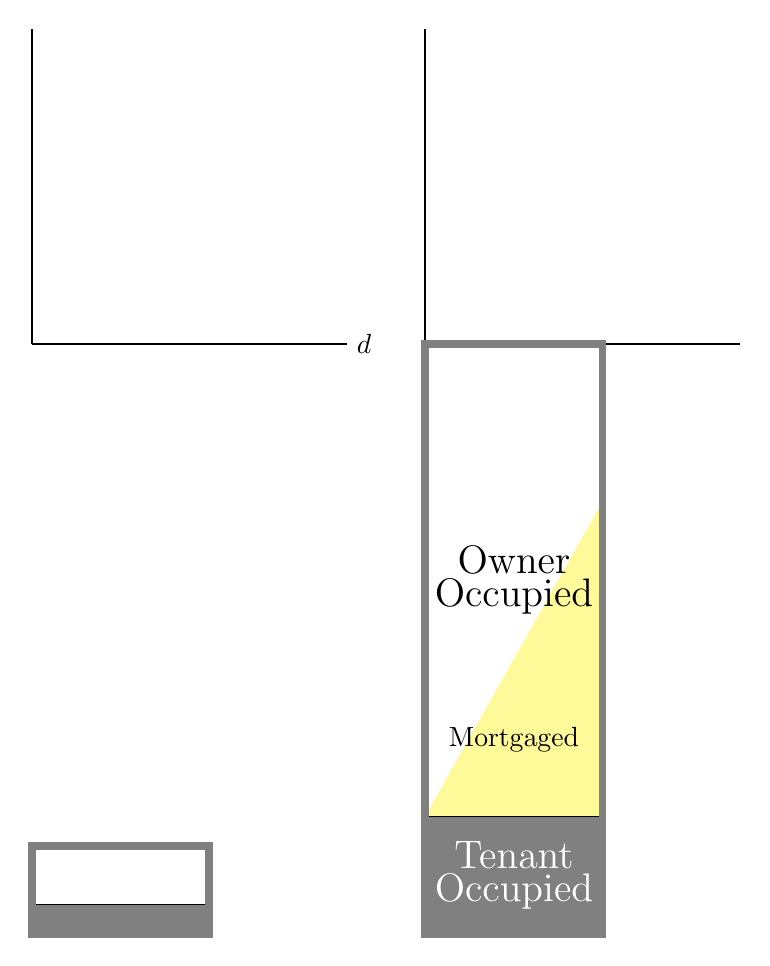
\begin{tikzpicture}[scale=.5]
%EXTENT  BEFORE
\draw[thick](0,0)--(0,8);
\draw[thick](0,0)--(8,0)node[right]{$d$};
%POPULATION BEFORE
\begin{scope}[shift={(0, -15cm)},scale=1.5]%population
\draw [fill=gray,] (0,0) rectangle (3,.5); %TENANT
\draw[line width= 1mm, black!50] (0,0) rectangle (3,1.5);
\end{scope}

% EXTENT AFTER
\begin{scope}[shift={(10cm, 0)}]
\draw[thick](0,0)--(0,8);
\draw[thick](0,0)--(8,0);
\end{scope}

%POPULATION AFTER
\begin{scope}[shift={(10, -15cm)},scale=1.5]%population
\draw [fill=gray,] (0,0) rectangle (3,2); %TENANT
\draw [fill=yellow!40] (0,2)--(3,2)--(3,7.33); --cycle;% 
\draw[line width= 1mm, black!50] (0,0) rectangle (3,10);
\node at (1.5,6)
    [text width=2.4cm, align=center]
    {\baselineskip=20pt\Large Owner Occupied};
\node at (2,3.3)
    [text width=2.4cm]
    {\baselineskip=20pt Mortgaged};
\node at (1.5,1)
    [text width=2.4cm, align=center, white]
    {\baselineskip=20pt\Large Tenant Occupied};
\end{scope}
 \end{tikzpicture}
 